\documentclass[../main.tex]{subfiles}
\graphicspath{{\subfix{../figures/}}}

\begin{document}
\section{UML中的动态建模技术}
\begin{itemize}
  \item \textbf{行为图}(Behavior diagram),描述系统的行为。包括\textbf{状态图}和\textbf{活动图}。
  \item \textbf{交互图}(Interactive diagram),描述对象间的交互关系。包括\textbf{顺序图},\textbf{合作图}。
\end{itemize}
\noindent \textbf{动态建模的应用}:
\begin{itemize}
  \item 不要对系统中的每个类都画状态图。状态图描述跨越多个用例的单个对象的行为,而不适合描述多个对象间的行为合作。
  \item 顺序图和合作图适合描述单个用例中几个对象的行为。其中顺序图突出对象间交互的顺序,而合作图的布局方法能更清楚地表示出对象之间静态的连接关系。当行为较为简单时,顺序图和合作图是最好的选择。
  \item 如果想显示跨越多用例或多线程的复杂行为,可考虑使用活动图。
\end{itemize}
\subsection{状态图}
\begin{itemize}
  \item 状态图(State Diagram)用来描述一个特定对象的所有可能状态及其引起状态转移的事件。
  \item 大多数面向对象技术都用状态图表示单个对象在其生命周期中的行为。
  \item 一个状态图包括一系列的状态以及状态之间的转移。
\end{itemize}
\textbf{状态}:
\begin{itemize}
  \item \textbf{初态}:状态图的起始点
  \item \textbf{终态}:状态图的终点
  \item \textbf{中间状态}:名字域和内部转移域.
    内部转移域是可选的,其中所列的动作将在对象处于该状态时执行,且该动作的执行并不改变对象的状态。
  \item \textbf{复合状态}:可以进一步细化的状态.
  \item 子状态间的关系:
    \begin{itemize}
      \item 或关系:在某一时刻仅可到达一个子状态。
      \item 与关系:在某一时刻可同时到达多个子状态。
    \end{itemize}
\end{itemize}
\begin{figure}[H]
  \begin{center}
    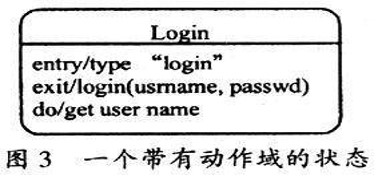
\includegraphics[width=0.25\textwidth]{6_1.jpg}
  \end{center}
\end{figure}
\begin{figure}[H]
  \begin{center}
    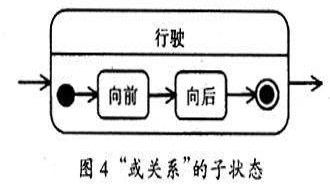
\includegraphics[width=0.25\textwidth]{6_2.jpg}
    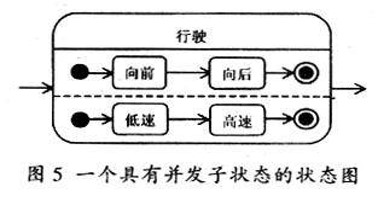
\includegraphics[width=0.25\textwidth]{6_3.jpg}
  \end{center}
\end{figure}
\begin{figure}[H]
  \begin{center}
    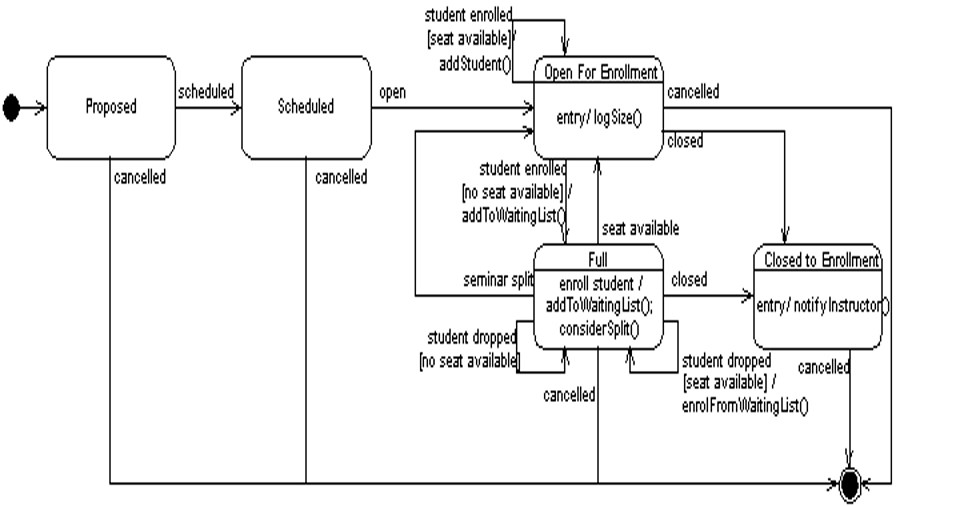
\includegraphics[width=0.75\textwidth]{6_4.jpg}
  \end{center}
\end{figure}
\subsection{活动图}
活动图(Activity Diagram)既可用来描述类(类的方法)的行为,也可以描述用例和对象内部的工作过程。
\begin{figure}[H]
  \begin{center}
    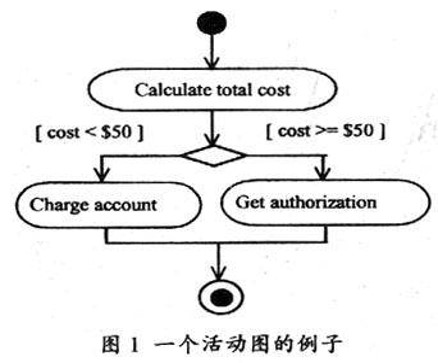
\includegraphics[width=0.35\textwidth]{6_5.jpg}
  \end{center}
\end{figure}
\textbf{活动图的模型元素}:
\begin{figure}[H]
  \begin{center}
    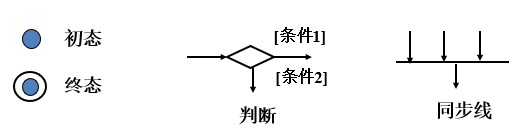
\includegraphics[width=0.55\textwidth]{6_6.jpg}
  \end{center}
\end{figure}
\noindent \textbf{转移}:
转移描述活动之间的关系,描述由于隐含事件引起的活动变迁,即转移可以连接各活动。
转移用带箭头的直线表示,可标注执行该转移的条件,无标注表示按顺序执行。

\noindent \textbf{泳道}:泳道进一步描述完成活动的对象,并聚合一组活动。泳道也是一种分组机制。
泳道可以直接显示动作在哪一个对象中执行,或显示的是一项组织工作的哪部分。
\begin{figure}[H]
  \begin{center}
    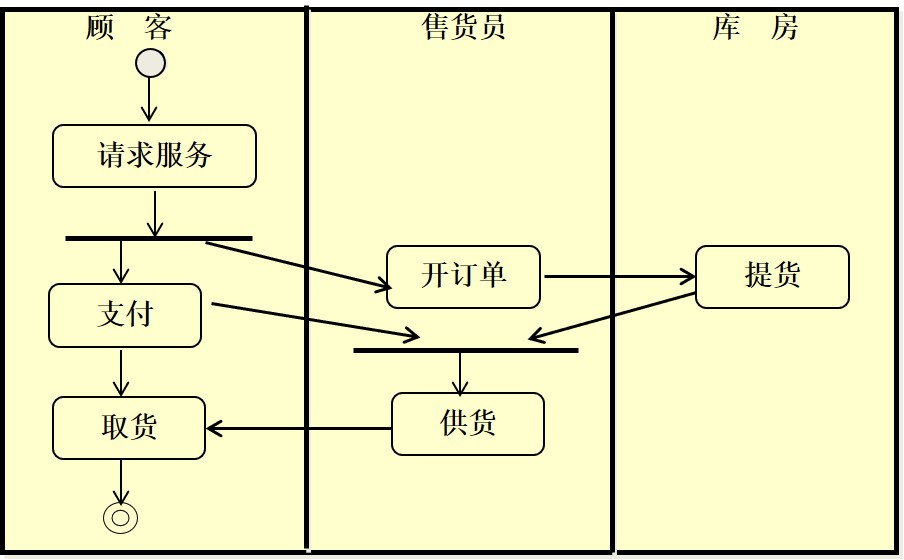
\includegraphics[width=0.35\textwidth]{6_7.jpg}
  \end{center}
\end{figure}
\textbf{对象流}:活动图中可以出现对象,对象作为活动的输入/输出,用虚箭头表示。
\begin{figure}[H]
  \begin{center}
    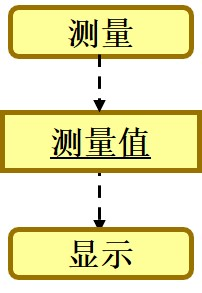
\includegraphics[width=0.15\textwidth]{6_8.jpg}
  \end{center}
\end{figure}
\textbf{控制图符}:活动图中可发送和接收信号,发送符号对应于与转移联系在一起的发送短句。接收符号也同转移联系在一起。
\begin{figure}[H]
  \begin{center}
    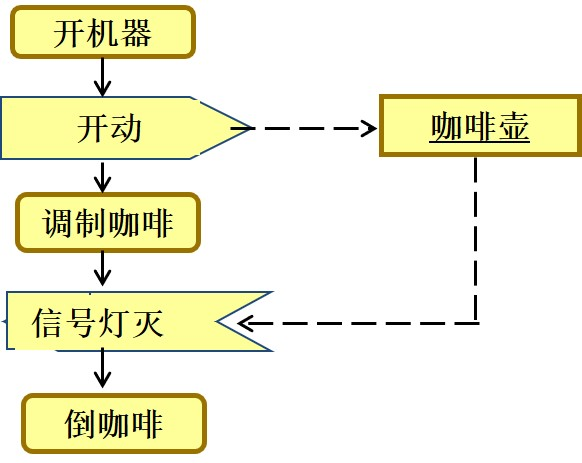
\includegraphics[width=0.35\textwidth]{6_9.jpg}
    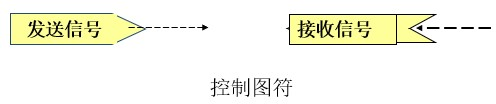
\includegraphics[width=0.50\textwidth]{6_10.jpg}
  \end{center}
\end{figure}
\textbf{发送和接收信号}:
活动图中可发送和接收信号,发送符号和接收符号对应于与转移联系在一起的发送短句。转移又分两种:发送信号的转移和接收信号的转移。发送和接收信号可以和消息的发送对象和接收对象联系在一起,如下图。
发送信号动作是一种特殊的动作,它表示从输入信息创建一个信号实例,然后发送到目标对象。发送信号动作可能触发状态的转换或者活动的执行。在发送信号动作时可以包含一组带有值的参数。由于信号是一种异步消息,所以发送方立即继续执行,所有的响应都将被忽略,并未返回给发送方.
\begin{figure}[H]
  \begin{center}
    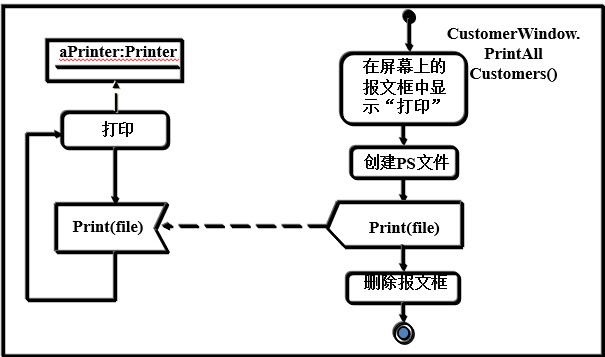
\includegraphics[width=0.45\textwidth]{6_11.jpg}
  \end{center}
\end{figure}
活动图中只有一个起点一个终点,表示方式和状态图一样,泳道被用来组合活动,通常根据活动的功能来组合。
\subsection{顺序图}
顺序图(Sequence Diagram)用来描述对象之间动态的交互关系,着重体现对象间消息传递的时间顺序。
顺序图的主要用途之一,是把用例表达的需求,转化为进一步、更加正式的、层次化的精细表达。

\textbf{顺序图构成}:一组对象(对象名和类名);对象生命线(时间轴);对象被激活;对象间的通信(消息).
\begin{figure}[H]
    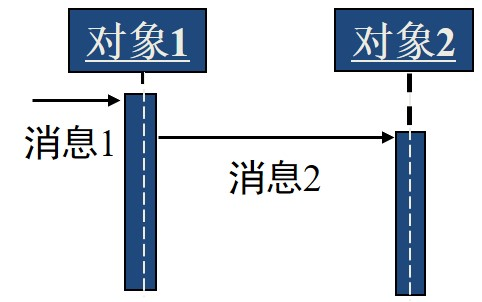
\includegraphics[width=0.45\textwidth]{6_12.jpg}
    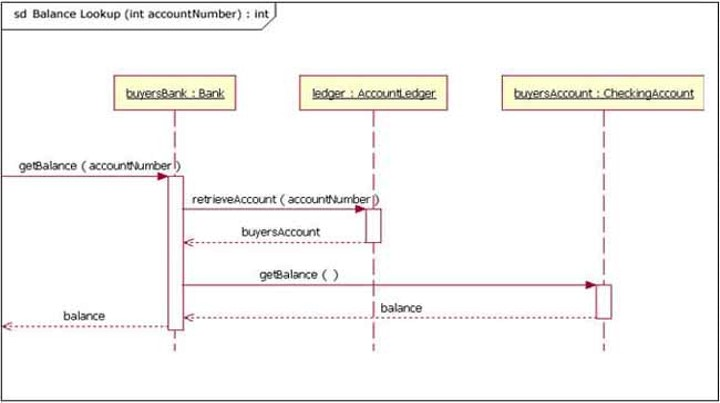
\includegraphics[width=0.55\textwidth]{6_13.jpg}
\end{figure}
\textbf{对象向自身发送消息}:
\begin{figure}[H]
    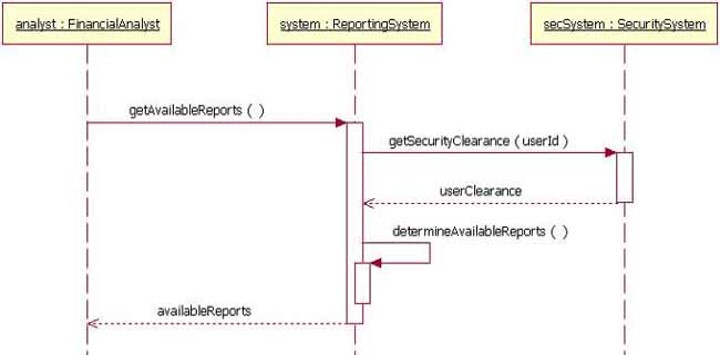
\includegraphics[width=0.75\textwidth]{6_14.jpg}
\end{figure}
\textbf{顺序图中的选择}:
\begin{figure}[H]
  \begin{center}
    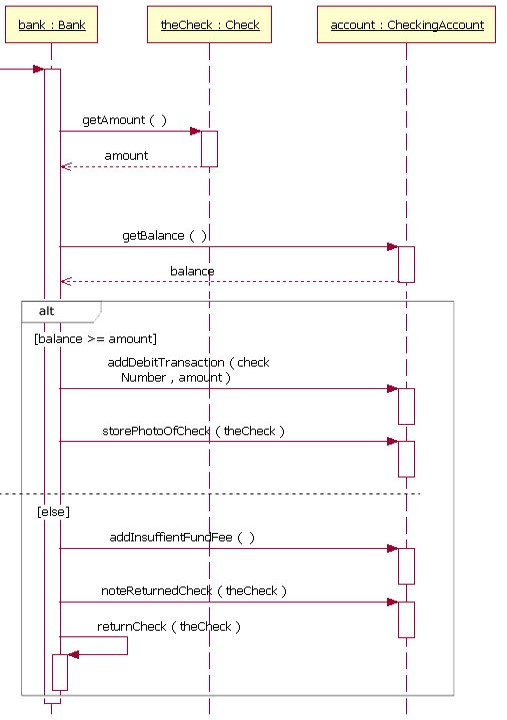
\includegraphics[width=0.45\textwidth]{6_15.jpg}
  \end{center}
\end{figure}
在顺序图中,还可以描述一个对象通过发送一条消息来创建另一个对象。
\begin{figure}[H]
  \begin{center}
    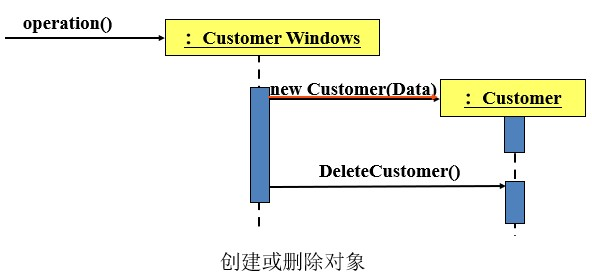
\includegraphics[width=0.55\textwidth]{6_16.jpg}
  \end{center}
\end{figure}
\subsection{合作图}
合作图(Collaboration Diagram)用于描述相互合作的对象间的交互关系和链接关系。着重体现交互对象间的静态链接关系。
\begin{figure}[H]
  \begin{center}
    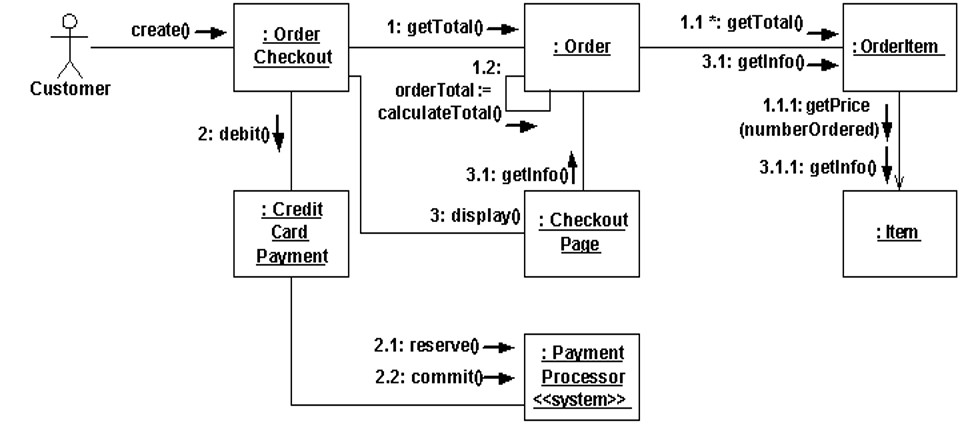
\includegraphics[width=0.75\textwidth]{6_17.jpg}
  \end{center}
\end{figure}
合作图中对象的外观与顺序图中的一样。如果一个对象在消息的交互中被创建,则可在对象名称之后标以\{new\}。类似地,如果一个对象在交互期间被删除,则可在对象名称之后标以\{destroy\}。
\begin{figure}[H]
  \begin{center}
    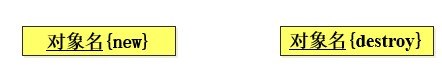
\includegraphics[width=0.45\textwidth]{6_18.jpg}
  \end{center}
\end{figure}
\textbf{消息}:在对象之间的静态链接关系上可标注消息。用标号表示, 标号有 3 种:
\begin{itemize}
  \item 顺序执行: 按整数大小执行. $ 1, 2, \cdots $.
  \item 嵌套执行: 标号中带小数点. $ 1.1, 1.2, 1.3, \cdots $.
  \item 并行执行: 标号中带小写字母. $ 1.1.1a, 1.1.1b, \cdots $.
\end{itemize}
\textbf{控制信息}:
\begin{itemize}
  \item 条件控制信息, 如: $ [x > y] $.
  \item 重复控制信息, 如: $ * [I=1..n] $.
\end{itemize}
\end{document}
